% ==========================================================================
% DRAFT (revised 2026-11-15).  Supplementary material for jc_beyond_linear.tex.
% Figures: simulations/sim_rotation_shear.py, sim_numerics_checks.py and the
% earlier scripts.
% Numbers of main-text equations, figures and tables are cited with \mainref{label}
% and come from jc_main_refs.tex: run tools/sync_supp_refs.py after renumbering.  Build: tectonic jc_beyond_linear_supp.tex
% ==========================================================================
\documentclass{iopjournal}
\usepackage{amsmath}
\usepackage{amssymb}
\usepackage{cite}
\graphicspath{{../figures/}{../../figures/}}
\fancyhead[L]{{\small \sf Supplementary material}}
\fancyhead[R]{N K Nguyen}
\newcommand{\nbar}{\bar{n}}
\newcommand{\ket}[1]{|#1\rangle}
\newcommand{\bra}[1]{\langle #1|}
\newcommand{\braket}[2]{\langle #1|#2\rangle}
% Generated by tools/sync_supp_refs.py from jc_beyond_linear.tex. Do not edit.
\makeatletter
\newcommand{\mainref}[1]{\@ifundefined{mainref@#1}{\textbf{??}}{\@nameuse{mainref@#1}}}
\@namedef{mainref@eq:H}{1}
\@namedef{mainref@eq:exact}{2}
\@namedef{mainref@eq:branches}{3}
\@namedef{mainref@eq:overlaps}{4}
\@namedef{mainref@eq:expansion}{5}
\@namedef{mainref@eq:rotation}{6}
\@namedef{mainref@eq:twobranch}{7}
\@namedef{mainref@eq:skeleton}{8}
\@namedef{mainref@eq:s}{9}
\@namedef{mainref@eq:shear}{10}
\@namedef{mainref@eq:lemma}{11}
\@namedef{mainref@eq:revival}{12}
\@namedef{mainref@eq:envelope}{13}
\@namedef{mainref@eq:parity}{14}
\@namedef{mainref@eq:fidelity}{15}
\@namedef{mainref@eq:negativity}{16}
\@namedef{mainref@eq:G}{17}
\@namedef{mainref@eq:nextorder}{18}
\@namedef{mainref@eq:purity}{19}
\@namedef{mainref@eq:residual}{20}
\@namedef{mainref@eq:visibility}{21}
\@namedef{mainref@fig:wigner}{1}
\@namedef{mainref@fig:envelopes}{2}
\@namedef{mainref@fig:portrait}{3}
\@namedef{mainref@fig:convergence}{4}
\@namedef{mainref@fig:loss}{5}
\@namedef{mainref@tab:orders}{1}
\@namedef{mainref@tab:test}{2}
\@namedef{mainref@sec:intro}{1}
\@namedef{mainref@sec:model}{2}
\@namedef{mainref@sec:orders}{3}
\@namedef{mainref@sec:rotation}{4}
\@namedef{mainref@sec:shear}{5}
\@namedef{mainref@sec:next}{6}
\@namedef{mainref@sec:numerics}{7}
\@namedef{mainref@sec:loss}{8}
\@namedef{mainref@sec:teaching}{9}
\@namedef{mainref@sec:conclusions}{10}
\makeatother

\renewcommand{\thesection}{S\arabic{section}}
\renewcommand{\theequation}{S\arabic{equation}}
\renewcommand{\thefigure}{S\arabic{figure}}
\renewcommand{\thetable}{S\arabic{table}}

\begin{document}

\articletype{Supplementary material}

\title{Supplementary material for ``Rotation and shear in the Jaynes--Cummings model: what the curvature of the Rabi spectrum does to revivals, cat states and entanglement''}

\author{Nguyen Khoi Nguyen}

\affil{Department of Electrical and Computer Engineering and Physics Department, Boston University, Boston, MA 02215, United States of America}

\begin{abstract}
Section~S1 derives the second-order results of the main text; section~S2 the corrections of order $1/\nbar$. Section~S3 describes the numerical methods and measures their errors against the exact solution. Section~S4 collects the limits of the asymptotic picture. Section~S5 treats other initial field states and the maps of the cat state under cavity loss. Section~S6 gives notes on the exercises. Equation, figure and table numbers without the prefix S refer to the main text.
\end{abstract}

\section{Second order: derivations}

\subsection{Notation}
The exact state is equation~(\mainref{eq:exact}), with phases $\theta_n = gt\sqrt{n+1}$ and Poisson weights $p_n = c_n^2$. As in the main text we write $n = \nbar + \delta n$ and $\varphi = gt/2\sqrt{\nbar}$, and use the phase space $a = (x+ip)/\sqrt{2}$, in which the vacuum has covariance matrix $\tfrac12 I$, with $I$ the $2\times2$ unit matrix.

\subsection{From the quadratic phase to the shear}
Near the coherent amplitude $\alpha = \sqrt{\nbar}$ write $a = \alpha + (\delta x + i\,\delta p)/\sqrt{2}$, so that $\delta x$ is the radial and $\delta p$ the tangential coordinate. To first order in the fluctuations
\begin{equation}
\hat{n} - \nbar = \alpha(\delta a + \delta a^\dagger) = \sqrt{2\nbar}\;\delta x,
\end{equation}
which reproduces $\mathrm{Var}(n) = 2\nbar\times\tfrac12 = \nbar$. The quadratic term of equation~(\mainref{eq:expansion}) is therefore $-\varphi\,\delta n^2/4\nbar = -\tfrac12\varphi\,\delta x^2$, and the corresponding factor in $\ket{\Phi_+}$ is the unitary $U = \exp(-\tfrac{i}{2}\varphi\,\delta x^2)$. Since $[\delta x^2, \delta p] = 2i\,\delta x$,
\begin{equation}
U^\dagger\,\delta p\,U = \delta p - \varphi\,\delta x,\qquad U^\dagger\,\delta x\,U = \delta x.
\end{equation}
The tangential coordinate is displaced in proportion to the radial one: a shear of magnitude $s = \varphi$, with the opposite sign for $\ket{\Phi_-}$. Applying it to the vacuum covariance matrix gives equation~(\mainref{eq:shear}), with the lower sign for $\ket{\Phi_+}$ and the upper sign for $\ket{\Phi_-}$ when the tangential coordinate is counted counter-clockwise. The classical argument of the main text is the same statement: the angular velocity is $\omega(R) = g/(\sqrt{2}\,R)$ at radius $R = \sqrt{2n}$, so $d\omega/dR = -\omega/R$ and a radial offset $\delta R$ accumulates the tangential offset $R\,\delta\omega\,t = -\omega t\,\delta R = -\varphi\,\delta R$.

The eigenvalues of $V(s)$ are $\tfrac12 e^{\pm2r}$ with $\cosh 2r = 1+s^2/2$, that is $\sinh r = s/2$. At $t_r/2$, $s = \pi/2$ and $e^{-2r} = 0.2364$, a reduction of 6.26~dB below the vacuum. These eigenvalues are the quadrature variances obtained by Gea-Banacloche [equations (B11)--(B13) of reference~\cite{S-gea1991}].

\subsection{The Gaussian overlap, in two languages}
For a Gaussian variable $u$ with zero mean and variance $\sigma^2$,
\begin{equation}
\big\langle e^{-i\mu u^2 + i\nu u}\big\rangle = \frac{1}{\sqrt{1+2i\mu\sigma^2}}\exp\!\left[-\frac{\nu^2\sigma^2}{2(1+2i\mu\sigma^2)}\right],
\label{eq:S-lemma}
\end{equation}
by completing the square; equation~(\mainref{eq:lemma}) is the case $\nu = 0$, $\sigma^2 = \nbar$. In phase space the equivalent statement is that two pure Gaussian states with covariance matrices $V_1$, $V_2$ whose centres differ by the vector $d$ have
\begin{equation}
|\braket{\psi_1}{\psi_2}|^2 = \frac{1}{\sqrt{\det(V_1+V_2)}}\exp\!\left[-\tfrac12\,d^{\rm T}(V_1+V_2)^{-1}d\right].
\label{eq:S-overlap}
\end{equation}
With equation~(\mainref{eq:shear}): $\det[V(s)+V(-s)] = 1+s^2$ and $\det[V(s)+\tfrac12 I] = 1+s^2/4$. These two determinants give the revival height, the parity amplitude and the cat fidelity.

\subsection{Poisson summation and the envelopes}
The inversion is $\mathrm{Re}\sum_n p_n e^{i\Lambda(n)}$ with $\Lambda(n) = 2gt\sqrt{n+1}$. The Poisson summation formula, $\sum_n f(n) = \sum_k\int f(n)\,e^{-2\pi ikn}\,dn$, turns the sum over integers into a sum over $k$ of integrals over a continuous $n$~\cite{S-fleischhauer1993}. Expand $\Lambda$ to second order about $\nbar$,
\begin{equation}
\Lambda(n) \simeq \Lambda_0 + \Lambda_1\,\delta n + \tfrac12\Lambda_2\,\delta n^2,\qquad
\Lambda_0 = 2gt\sqrt{\nbar+1},\quad \Lambda_1 = \frac{gt}{\sqrt{\nbar+1}},\quad \Lambda_2 = -\frac{gt}{2(\nbar+1)^{3/2}},
\end{equation}
and replace $p_n$ by a Gaussian of variance $\nbar$. Equation~(\ref{eq:S-lemma}) then gives the $k$th term
\begin{equation}
T_k(t) = \frac{e^{i(\Lambda_0-2\pi k\nbar)}}{\sqrt{1-i\Lambda_2\nbar}}\exp\!\left[-\frac{\nbar(\Lambda_1-2\pi k)^2}{2(1-i\Lambda_2\nbar)}\right],
\label{eq:S-Sk}
\end{equation}
and $\langle\sigma_z\rangle\simeq\mathrm{Re}\sum_{k\geq0}T_k$. To leading order $\Lambda_1 = 2\varphi$ and $-\Lambda_2\nbar = \varphi$, so $|T_k|$ is the $k$th term of equation~(\mainref{eq:envelope}); the envelopes drawn in figures~\mainref{fig:envelopes} and \mainref{fig:portrait} use equation~(\ref{eq:S-Sk}) as it stands. The term $k$ is appreciable only where $\Lambda_1\approx 2\pi k$, i.e.\ near $t = kt_r$: each revival is one term of the Poisson sum, and its height and width are those of an overlap of two Gaussians sheared by $\pm k\pi$.

For the parity the summand carries the extra factor $(-1)^n = e^{-i\pi n}$, which shifts $k$ to $k+\tfrac12$: the parity is $\mathrm{Re}\sum_{k\geq0}T_{k+1/2}$, with bumps at half-odd multiples of $t_r$.

Equation~(\ref{eq:S-Sk}) is accurate to relative order $1/\nbar$ only at the centre of a bump. On the flanks the error of the envelope is of relative order $\nbar^{-1/2}$: for the first revival at $\nbar = 100$ it is 3\% at one standard deviation from the centre, against 0.1\% at the centre. Equation~(\mainref{eq:envelope}) as written, with $\nbar$ in place of $\nbar+1$, is centred at $kt_r$ rather than at $2\pi k\sqrt{\nbar+1}/g$ and is about twice as far off on the flanks (6\%). The phase of the fast oscillation is likewise correct only to order $\nbar^{-1/2}$ away from the centre: over $0<t<2.5\,t_r$ the largest pointwise difference between $\mathrm{Re}\sum_k T_k$ and the exact inversion is 0.26, 0.16 and 0.07 for $\nbar = 10$, 25 and 100.

\subsection{Fidelity with a cat state}
At $t_r/2$ the field is, up to corrections of order $1/\nbar$ (section~S2), the pure state $(\ket{\Phi_-}+\ket{\Phi_+})/\sqrt{2}$ [equation~(\mainref{eq:twobranch}) with $\varphi = \pi/2$], whose components are centred at $\mp i\alpha$. Its squared overlap with the cat state $(\ket{{-}i\alpha}+e^{i\theta}\ket{i\alpha})/\sqrt2$ is, for well-separated components and after the relative phase $\theta$ is chosen optimally, the squared overlap of one sheared component with the coherent state at its centre, so $F_{\rm cat} = (1+s^2/4)^{-1/2}$ with $s = \pi/2$. More generally the fidelity of a single component with a coherent state at time $t$ is $(1+\varphi^2/4)^{-1/2}$, the peak value of the $Q$ function of reference~\cite{S-gea1991}. At finite $\nbar$ the result depends on the family of cat states allowed. Table~\mainref{tab:test} uses states proportional to $\ket{\beta}+e^{i\theta}\ket{{-}\beta}$ and approaches the limit from below; if the two coherent amplitudes and their weights are optimized independently the fidelity is 0.802, 0.793 and 0.788 for $\nbar = 10$, 25 and 100, approaching the same limit from above.

\subsection{Wigner negativity}
For $\ket{\psi} = (\ket{\psi_1}+\ket{\psi_2})/\sqrt2$ with well-separated components, $W = \tfrac12W_1+\tfrac12W_2+\mathrm{Re}\,W_{12}$, where $W_{12}$ is the cross Wigner function. Its modulus is a smooth envelope and its phase advances linearly across the envelope, producing fringes. If there are many fringes under the envelope, $\int|\mathrm{Re}\,W_{12}| = (2/\pi)\int|W_{12}|$, since $2/\pi$ is the mean of $|\cos|$. The modulus can be written as an overlap: $|W_{12}(z)| = \pi^{-1}|\bra{\psi_1}D(2z)\Pi\ket{\psi_2}|$ with $D$ a displacement and $\Pi$ the parity operator, so for Gaussian components equation~(\ref{eq:S-overlap}) gives a Gaussian in $z$ whose integral is
\begin{equation}
\int|W_{12}|\,dx\,dp = \big[\det(V_1+V_2)\big]^{1/4}.
\end{equation}
For two identical coherent states this is one and $\delta = 2/\pi$. The two JC components at $t_r/2$ sit at opposite points of the circle, so their (radial, tangential) frames differ by a rotation through $\pi$, which leaves a covariance matrix unchanged; in a common frame their covariance matrices are $V(s)$ and $V(-s)$, the determinant is $1+s^2$, and the integral is $(1+s^2)^{1/4}$, which is equation~(\mainref{eq:negativity}). Note that $(1+s^2)^{1/4}$ is the reciprocal of the parity amplitude: the interference term has a fixed $L^2$ norm, so a lower central fringe ($W(0) = \langle(-1)^{\hat n}\rangle/\pi$) must be spread over a larger area, and $\int|W|$ grows.

Table~\ref{tab:S-delta} shows the approach to the limit, which is not monotonic: $\delta$ overshoots to 0.881 near $\nbar = 25$, where the components themselves still contribute negativity, dips to about 0.8665 between $\nbar = 100$ and 200, and then approaches 0.8687 from below as $-0.5/\nbar$.

\begin{table}
\centering
\caption{Wigner negativity of the reduced field at $t_r/2$ from the Fourier method of section~S3.4, converged with respect to the grid spacing to the digits shown for $\nbar\leq400$ and to $2\times10^{-5}$ beyond. Limit: $(2/\pi)(1+\pi^2/4)^{1/4} = 0.86872$.}
\begin{tabular}{cccccccccc}
\hline
$\nbar$ & 4 & 10 & 25 & 50 & 100 & 200 & 400 & 1600 & 6400 \\
$\delta$ & 0.6471 & 0.8505 & 0.8805 & 0.8727 & 0.8672 & 0.8666 & 0.8675 & 0.86841 & 0.86864 \\
\hline
\end{tabular}
\label{tab:S-delta}
\end{table}

\section{Corrections of order $1/\nbar$}

\subsection{The amplitudes $Z_k$}
At $t = kt_r = 2\pi k\sqrt{\nbar}/g$, $Z_k = \sum_n p_n\exp[i\Lambda(n) - 2\pi ikn]$ with $\Lambda(n) = 4\pi k\sqrt{\nbar(n+1)}$. Put $n = \nbar+\delta n$, $\xi = \delta n/\sqrt{\nbar}$ and $\epsilon = \nbar^{-1/2}$. Expanding the square root to fourth order, the linear terms cancel and
\begin{equation}
\Lambda - 2\pi kn = 2\pi k(\nbar+1) - \frac{K}{2}\xi^2 + \epsilon K\Big(\frac{\xi^3}{4}-\xi\Big) + \epsilon^2K\Big(-\frac12+\frac34\xi^2-\frac{5}{32}\xi^4\Big) + O(\epsilon^3),\qquad K = \pi k.
\end{equation}
The Poisson weight, continued to real $n$ with Stirling's series, is
\begin{equation}
p(\nbar+\delta n)\,d(\delta n) = \frac{d\xi}{\sqrt{2\pi}}\exp\!\Big[-\frac{\xi^2}{2} + \epsilon\Big(\frac{\xi^3}{6}-\frac{\xi}{2}\Big) + \epsilon^2\Big(-\frac{\xi^4}{12}+\frac{\xi^2}{4}-\frac1{12}\Big) + O(\epsilon^3)\Big].
\end{equation}
The leading integrand is a Gaussian of complex variance $v = (1+iK)^{-1}$, giving $G(k) = v^{1/2}$. Writing the order-$\epsilon$ exponent as $a_1 = b_1\xi+b_3\xi^3$ with $b_1 = -\tfrac12-iK$, $b_3 = \tfrac16+\tfrac{i}{4}K$, and the order-$\epsilon^2$ exponent as $a_2$, the terms odd in $\xi$ average to zero and
\begin{equation}
Z_k = e^{2\pi ik(\nbar+1)}\,v^{1/2}\Big[1 + \epsilon^2\big(\langle a_2\rangle + \tfrac12\langle a_1^2\rangle\big)\Big],\qquad
\langle\xi^2\rangle = v,\ \langle\xi^4\rangle = 3v^2,\ \langle\xi^6\rangle = 15v^3.
\end{equation}
Collecting terms,
\begin{equation}
j(k) = \langle a_2\rangle+\tfrac12\langle a_1^2\rangle = -\frac{K(8K^2+3)}{96\,(K-i)^3},
\end{equation}
which is equation~(\mainref{eq:nextorder}). Its real part, $-K^2(K^2-3)(8K^2+3)/96(1+K^2)^3$, changes sign at $K = \sqrt3$: the leading formula underestimates $|Z_k|$ for $k<0.55$ and overestimates it beyond. Table~\ref{tab:S-j} compares $j(k)$ with $\nbar\,(Z_k/Z_k^{(0)}-1)$ from the exact sum.

\begin{table}
\centering
\caption{The coefficient $j(k)$ of equation~(\mainref{eq:nextorder}) against $\nbar(Z_k/Z_k^{(0)}-1)$ evaluated from the exact sum, where $Z_k^{(0)} = e^{2\pi ik(\nbar+1)}G(k)$.}
\begin{tabular}{cccc}
\hline
$k$ & $j(k)$ & exact, $\nbar = 25$ & exact, $\nbar = 400$ \\
\hline
$1/2$ & $\phantom{-}0.0075-0.0571i$ & $\phantom{-}0.0075-0.0572i$ & $\phantom{-}0.0075-0.0571i$ \\
$1$ & $-0.0451-0.0597i$ & $-0.0450-0.0595i$ & $-0.0451-0.0597i$ \\
$3/2$ & $-0.0642-0.0466i$ & $-0.0584-0.0524i$ & $-0.0642-0.0466i$ \\
$2$ & $-0.0721-0.0369i$ & $-0.0719+0.0342i$ & $-0.0721-0.0369i$ \\
\hline
\end{tabular}
\label{tab:S-j}
\end{table}

For $k = 3/2$ and 2 the agreement at $\nbar = 25$ is poor: those bumps overlap their neighbours (section~S4), and a single term of the Poisson sum no longer describes the amplitude.

\subsection{Purity between collapse and revival}
The reduced field state has rank two, $\rho_{\rm field} = \ket{A}\bra{A}+\ket{B}\bra{B}$, with $\ket{A} = \sum_n c_n\cos\theta_n\ket{n}$ (atom in $\ket{e}$) and $\ket{B} = -i\sum_m c_{m-1}\sin\theta_{m-1}\ket{m}$ (atom in $\ket{g}$). Hence
\begin{equation}
\mathcal{P} = p_e^2+p_g^2+2|\braket{A}{B}|^2,\qquad p_e = \braket{A}{A},\quad p_g = \braket{B}{B} = 1-p_e.
\end{equation}
Using $\cos\theta\sin\theta' = \tfrac12[\sin(\theta+\theta')-\sin(\theta-\theta')]$,
\begin{equation}
\braket{A}{B} = -\frac{i}{2}\sum_m c_mc_{m-1}\big[\sin(\theta_m+\theta_{m-1}) - \sin(\theta_m-\theta_{m-1})\big].
\end{equation}
The first sum has the same structure as the inversion and is negligible between collapse and revival, where also $p_e = p_g = \tfrac12$. In the second, $\theta_m-\theta_{m-1} = gt/(\sqrt{m+1}+\sqrt m) \simeq \varphi\sqrt{\nbar/(m+\tfrac12)}$ and $c_mc_{m-1} = p_m\sqrt{m/\nbar}$. With $y = m-\nbar$, the weights $p_m\sqrt{m/\nbar}$ sum to $1-1/8\nbar$ and have $\langle y\rangle = \tfrac12$, $\langle y^2\rangle = \nbar$ to the order needed, and expanding the sine,
\begin{equation}
\sum_m c_mc_{m-1}\sin(\theta_m-\theta_{m-1}) = \Big(1-\frac{1}{8\nbar}\Big)\Big[\sin\varphi\Big(1-\frac{\varphi^2}{8\nbar}\Big) - \frac{\varphi\cos\varphi}{8\nbar}\Big] + O(\nbar^{-2}).
\end{equation}
Squaring and inserting in $\mathcal{P} = \tfrac12+2|\braket{A}{B}|^2$ gives equation~(\mainref{eq:purity}). The Bloch vector given by Kennedy \textit{et al}~\cite{S-kennedy2010} for the collapsed interval, of length $|\sin\varphi|\,e^{-\varphi^2/8\nbar}$ in our notation, reproduces the leading term and the term in $\varphi^2\sin^2\varphi$ of equation~(\mainref{eq:purity}); the other terms of order $1/\nbar$ are not contained in it. The same Gaussian factor is the loss of purity found in reference~\cite{S-gea1992}. The term $\varphi^2\sin^2\varphi/8\nbar$ is the spread of the atomic states $\ket{\chi_\mp}$ across the photon-number distribution; the term $\sin^2\varphi/8\nbar$ comes from the mismatch between $c_m$ and $c_{m-1}$. For a pure atom--field state the eigenvalues of the reduced atomic state are $\tfrac12(1\pm\sqrt{2\mathcal{P}-1})$, which gives the entropy. Table~\ref{tab:S-purity} tests equation~(\mainref{eq:purity}).

\begin{table}
\centering
\caption{Field purity: exact / equation~(\mainref{eq:purity}). The formula holds between the collapse and the revival; its failure at $\varphi = 3\pi/4$ for $\nbar\leq25$ marks the arrival of the revival.}
\begin{tabular}{cccccc}
\hline
$\varphi$ & $\pi/4$ & $3\pi/8$ & $\pi/2$ & $5\pi/8$ & $3\pi/4$ \\
\hline
$\nbar = 10$ & 0.7343 / 0.7350 & 0.8952 / 0.8961 & 0.9598 / 0.9567 & 0.8713 / 0.8837 & 0.7683 / 0.7238 \\
$\nbar = 25$ & 0.7439 / 0.7440 & 0.9144 / 0.9145 & 0.9827 / 0.9827 & 0.9104 / 0.9095 & 0.7261 / 0.7395 \\
$\nbar = 100$ & 0.7485 / 0.7485 & 0.9237 / 0.9237 & 0.9957 / 0.9957 & 0.9225 / 0.9225 & 0.7474 / 0.7474 \\
\hline
\end{tabular}
\label{tab:S-purity}
\end{table}

\subsection{Loss with amplitude decay}
The exponent of equation~(\mainref{eq:visibility}) is that of reference~\cite{S-meunier2006}; the model with loss is analysed more completely there and in reference~\cite{S-gea1993}. A simple refinement includes the decay $\alpha\to\alpha e^{-\kappa t/2}$ of the amplitude in the decoherence rate, $\Gamma(t) = 2\kappa\nbar e^{-\kappa t}\sin^2\omega t$ with $\omega = g/2\sqrt{\nbar}$. Its integral up to $T = \pi/2\omega$ is
\begin{equation}
\int_0^T\Gamma\,dt = \nbar\big(1-e^{-\kappa T}\big) - \frac{\kappa^2\nbar\,(1+e^{-\kappa T})}{\kappa^2+4\omega^2},
\end{equation}
which reduces to $\pi\kappa\nbar^{3/2}/g$ for $\kappa T\ll1$. For $\nbar = 10$ the visibilities $\exp(-\int\Gamma)$ are 0.396, 0.177 and 0.030 at $\kappa/g = 0.01$, 0.02, 0.05, against the simulated 0.403, 0.168, 0.025 and the 0.370, 0.137, 0.007 of equation~(\mainref{eq:visibility}). The refinement removes most of the discrepancy but still ignores the change of the rotation rate as the field decays.

\section{Numerical methods and their limits}

Three levels of computation are used. (i) \emph{Exact sums}: equation~(\mainref{eq:exact}) evaluated directly, with the Poisson weights from a library routine and the sum cut where the weight is below $10^{-30}$ ($n\leq\nbar+14\sqrt{\nbar}+40$). This is the reference for everything else. (ii) \emph{Schr\"{o}dinger equation}: the state vector in a Fock space truncated at $N_{\rm cav}$, propagated with QuTiP~5.2~\cite{S-johansson2012, S-johansson2013, S-lambert2026} (\texttt{sesolve}/\texttt{mesolve}, Adams method). (iii) \emph{Master equation}: the density matrix, $(2N_{\rm cav})^2$ elements, for the runs with loss. Figure~\ref{fig:S-numerics} measures the error of level (ii) and of the phase-space integration against level (i).

\begin{figure}
\centering
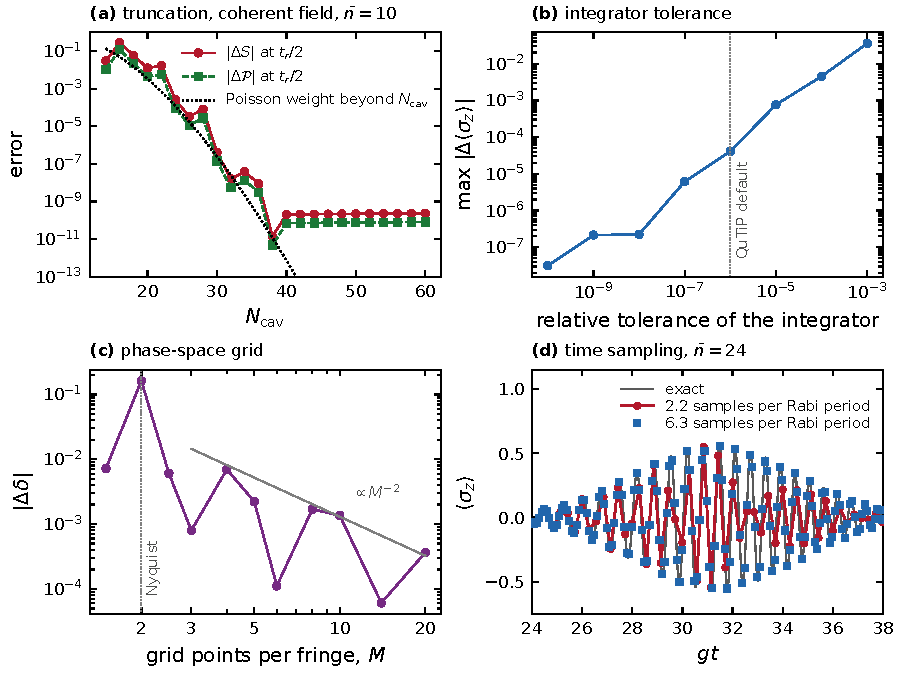
\includegraphics[width=\textwidth]{fig_numerics_checks.pdf}
\caption{Numerical errors measured against the exact solution. (a) Error of the entropy and purity at $t_r/2$ when the field is truncated at $N_{\rm cav}$ ($\nbar = 10$); dotted: Poisson weight beyond $N_{\rm cav}$. The floor at $10^{-10}$ is the integrator tolerance used for this test. (b) Largest error of the inversion over $0<t<1.5\,t_r$ against the relative tolerance of the integrator (absolute tolerance $10^{-2}$ times smaller), for $\nbar = 10$. (c) Error of the Wigner negativity at $t_r/2$ against the number $M$ of grid points per interference fringe ($\nbar = 10$); the grey line has slope $-2$. (d) The first revival for $\nbar = 24$: exact inversion (line) and the same curve sampled at 2.2 (connected circles) and 6.3 (squares) points per Rabi period.}
\label{fig:S-numerics}
\end{figure}

\subsection{Truncation}
For the coherent field the error follows the Poisson weight outside the truncated space to within an order of magnitude [figure~\ref{fig:S-numerics}(a)]: for $\nbar = 10$ it is $1.3\times10^{-2}$ in the entropy at $N_{\rm cav} = 20$, $2.6\times10^{-4}$ at 24, $4\times10^{-7}$ at 30 and $4\times10^{-8}$ at 34. A safe rule is $N_{\rm cav}\geq\nbar+8\sqrt{\nbar}$. The rule is specific to Poisson statistics. The weight beyond $N_{\rm cav}$ is $(\nbar/(\nbar+1))^{N_{\rm cav}}$ for a thermal field and falls even more slowly for a squeezed vacuum (table~\ref{tab:S-tails}). Truncating such a state does not merely lose accuracy: it changes the state, lowering $\langle n\rangle$ from 10 to 9.57 (thermal) or 8.23 (squeezed) at $N_{\rm cav} = 50$. We build the squeezed vacuum from its exact Fock amplitudes rather than by exponentiating a truncated generator. Conservation of the trace is not a convergence test, since the truncated dynamics is still unitary.

\begin{table}
\centering
\caption{Photon-number weight beyond $N_{\rm cav}$ for three fields with $\nbar = 10$.}
\begin{tabular}{cccc}
\hline
$N_{\rm cav}$ & coherent & thermal & squeezed vacuum \\
\hline
50 & $1.9\times10^{-19}$ & $8.5\times10^{-3}$ & $3.0\times10^{-2}$ \\
150 & $<10^{-100}$ & $6.2\times10^{-7}$ & $1.6\times10^{-4}$ \\
300 & $<10^{-100}$ & $3.8\times10^{-13}$ & $9.2\times10^{-8}$ \\
\hline
\end{tabular}
\label{tab:S-tails}
\end{table}

\subsection{Integrator tolerance}
The error of the inversion is proportional to the relative tolerance over five decades [figure~\ref{fig:S-numerics}(b)]: $3.6\times10^{-2}$ at $10^{-3}$, $4.1\times10^{-5}$ at QuTiP's default $10^{-6}$, $2\times10^{-7}$ at $10^{-8}$. The default is ample for a figure and for three-digit numbers. It is not enough to verify a $1/\nbar^2$ law at $\nbar = 100$, where the quantity of interest is $10^{-7}$ or smaller; for that we use the exact sums.

\subsection{Time sampling}
The fastest Rabi frequency carrying weight is about $2g\sqrt{\nbar+3\sqrt{\nbar}}$, and the entropy and purity oscillate at twice the Rabi frequency. A trace sampled near two points per period is aliased into a slow, smooth and entirely spurious envelope [figure~\ref{fig:S-numerics}(d)]; an earlier version of one of our own figures suffered from exactly this. We sample every plotted curve at 20 or more points per period of its fastest component.

\subsection{Wigner function and its negativity}
QuTiP evaluates $W$ on a grid from the Fock-basis density matrix by a Clenshaw recurrence over Laguerre polynomials, at a cost proportional to $N_{\rm cav}^2$ times the number of grid points. The cat fringes have period $\pi/\sqrt{2\nbar}$ while the state extends over $\sqrt{2\nbar}$, so a grid covering the state at fixed resolution per fringe has of order $\nbar^2$ points and the cost grows asymptotically as $\nbar^4$. At ten points per fringe it is 5~s at $\nbar = 25$, 80~s at 64 and 340~s at 100 on a laptop.

The negativity needs $\int|W|$, and $|W|$ has a kink wherever $W$ changes sign. The trapezoidal rule, spectrally accurate for the smooth $W$ itself, then converges only as the inverse square of the number $M$ of points per fringe, with an error whose sign and size depend on where the grid falls relative to the fringes [figure~\ref{fig:S-numerics}(c)]: 0.16 at $M = 2$, where the samples can sit on the zeros, up to $7\times10^{-3}$ for $M\leq5$, about $10^{-3}$ at $M = 10$. The maps for $\nbar = 10$ use $M = 14$, for which $\delta$ is stable to better than $10^{-3}$. The sweep of section~S3.6 uses a fixed spacing of 0.055, that is, $M$ from 13 at $\nbar = 10$ to 8 at $\nbar = 25$; its lossless values differ from the converged ones by up to $2\times10^{-3}$. A non-integer $M$ is preferable to an integer one, because it lets the sampling phase drift across the envelope.

For the convergence study we use a faster route that exploits the structure of the problem. The reduced state has rank two, so $W$ is the sum of two pure-state Wigner functions, each the Fourier transform over $y$ of $\psi^*(x+y)\psi(x-y)$, where $\psi(x) = \sum_n a_n\phi_n(x)$ is built from the oscillator eigenfunctions $\phi_n$ by their three-term recurrence. At $t_r/2$ the components lie on the $p$ axis, so $\psi$ is confined to $|x|<16$ for any $\nbar$ and only the spacing must follow the fringe period. The cost grows roughly as $\nbar$ rather than $\nbar^4$: 0.5~s at $\nbar = 100$ with 32 points per fringe, 4~s at $\nbar = 6400$ with 12. The two methods agree to $5\times10^{-4}$ at $\nbar = 10$ ($\delta = 0.8505$).

\subsection{Entanglement measures}
The entropy follows from the two eigenvalues of the reduced atomic state. For a pure atom--field state with Schmidt probabilities $\lambda_{1,2}$ the logarithmic negativity is $\log_2(1+2\sqrt{\lambda_1\lambda_2})$, a function of the same eigenvalues, so it adds nothing to the entropy; it becomes informative, and requires diagonalizing the $2N_{\rm cav}$-dimensional partial transpose at every time step, only when the global state is mixed (section~S5).

\subsection{Master equation and cost}
With loss the density matrix has $(2N_{\rm cav})^2$ elements with $N_{\rm cav}\approx3\nbar+20$, and the number of integrator steps to $t_r/2$ is proportional to the number of Rabi periods, $\nbar$. The sweep behind figure~\mainref{fig:loss} covers 16 values of $\nbar$ from 1 to 25 and 25 values of $\kappa/g$ (zero and 24 values spaced logarithmically from $10^{-3}$ to 0.2), and takes about six minutes. The logarithmic spacing matters: because the threshold falls roughly as $\nbar^{-3/2}$, a linear grid of step 0.01 cannot resolve it for $\nbar>15$, and a fit to such data gave us a spurious exponent of $-1.14$ before the grid was refined. Table~\ref{tab:S-cost} summarizes the scaling.

\begin{table}
\centering
\caption{How the cost of each computation grows with the mean photon number.}
\begin{tabular}{lll}
\hline
Computation & Cost & Reach in this work \\
\hline
Exact sums for inversion, parity, purity, $Z_k$ & $\nbar$ per time point & $\nbar = 400$ \\
Cat fidelity (optimization over a cat) & $\nbar$ per evaluation & $\nbar = 400$ \\
Negativity, Fourier method at $t_r/2$ & $\nbar$ & $\nbar = 6400$ \\
Schr\"{o}dinger equation to $t_r$ & $\nbar^2$ & $\nbar = 36$ \\
Wigner function on a full grid & $\nbar^4$ & $\nbar = 100$ \\
Master equation to $t_r/2$ & $\nbar^3$ & $\nbar = 25$ \\
\hline
\end{tabular}
\label{tab:S-cost}
\end{table}

\section{Limits of the asymptotic picture}

\textit{Small $\nbar$.} The bumps of equation~(\mainref{eq:envelope}) have width $\sigma_\varphi = \sqrt{(1+\varphi^2)/4\nbar}$ and spacing $\pi$. The collapse and first revival are separated only if $\sqrt{(1+\pi^2)/4\nbar}\ll\pi/2$, i.e.\ $\nbar\gg1$; in practice the constants of table~\mainref{tab:test} are within 0.5\% of their limits for $\nbar\geq16$, except the negativity, the slowest to converge (1.4\% above its limit at $\nbar = 25$, 0.2\% below at $\nbar = 100$). At $\nbar = 10$ the scaled impurity is still 7\% off.

\textit{Late revivals.} Bumps $k$ and $k+1$ overlap when $4\sigma_\varphi\approx\pi$, i.e.\ $k\approx\sqrt{\nbar}/2$. Beyond that the inversion is a sum of several terms of the Poisson series with comparable weight and the single-overlap picture no longer applies, although equation~(\ref{eq:S-Sk}) summed over $k$ remains a fair description of the envelope.

\textit{Non-Gaussian components.} Table~\ref{tab:S-squeezing} shows the covariance of one component from the exact amplitudes. Twice the off-diagonal element, which is the shear, is correct to about 10\% already at $\nbar = 10$. The determinant, which is $1/4$ for any pure Gaussian, is not: at $\nbar = 10$ and $t = t_r$ it is ten times too large. The component is bent along the circle of radius $\sqrt{2\nbar}$ (figure~\mainref{fig:wigner}), which adds a radial variance of order $1/\nbar$ ($1.9/\nbar$ at $t_r/2$, to be compared with the smallest eigenvalue 0.118 of $V(\pi/2)$). Quantities defined by overlaps are insensitive to this; the squeezing, which is the smallest eigenvalue of the covariance matrix, is very sensitive.

\begin{table}
\centering
\caption{One field component, from the exact amplitudes, in (radial, tangential) coordinates: magnitude of twice the off-diagonal element of its covariance matrix (prediction: $s$; the element is positive for $\ket{\Phi_-}$ and negative for $\ket{\Phi_+}$ when the tangential coordinate is counted counter-clockwise), the determinant (prediction: $0.25$) and the smallest eigenvalue relative to the vacuum value $1/2$, in decibels (prediction in the last row).}
\begin{tabular}{cccc}
\hline
 & $t_r/4$ ($s = \pi/4$) & $t_r/2$ ($s = \pi/2$) & $t_r$ ($s = \pi$) \\
\hline
$\nbar = 10$ & 0.70, 0.268, $-2.7$ dB & 1.43, 0.394, $-3.6$ dB & 2.78, 2.43, $+0.7$ dB \\
$\nbar = 100$ & 0.78, 0.252, $-3.3$ dB & 1.57, 0.267, $-5.9$ dB & 3.21, 0.656, $-6.4$ dB \\
$\nbar = 400$ & 0.78, 0.251, $-3.3$ dB & 1.57, 0.254, $-6.2$ dB & 3.16, 0.354, $-9.2$ dB \\
prediction & 0.79, 0.250, $-3.3$ dB & 1.57, 0.250, $-6.3$ dB & 3.14, 0.250, $-10.7$ dB \\
\hline
\end{tabular}
\label{tab:S-squeezing}
\end{table}

\textit{What the squeezing refers to.} The 6.3~dB is the squeezing of one component. At $t_r/2$ the two atomic states $\ket{\chi_\mp}$ coincide, so a measurement of the atom cannot select one component there; the reduced field is a superposition of two displaced components and its quadrature variances are dominated by their separation. A single squeezed component is obtained as the reduced field itself when the atom starts in $(\ket{e}+\ket{g})/\sqrt2$, for which only one component is populated~\cite{S-gea1991} (exercise 7).

\section{Other initial fields, and maps of the decohering cat}

The rotation-and-shear picture relies on a photon-number distribution narrow compared with its mean. Figure~\ref{fig:S-states} shows what happens otherwise, for four initial fields with $\nbar = 10$, integrated numerically ($N_{\rm cav} = 50$, 150, 300, 50 for coherent, thermal, squeezed vacuum and Fock). A thermal field, whose distribution has width $\nbar$, dephases within a Rabi period and never rephases cleanly. Its reduced atomic entropy saturates near 1~bit, but the global state is mixed, and the entropy of a subsystem then no longer measures entanglement: it registers classical correlations with the field as well. The logarithmic negativity $E_{\mathcal N} = \log_2\|\rho^{T_{\rm atom}}\|_1$, which vanishes for separable states, stays near 0.23. This is a useful counterexample to the habit of reading the reduced entropy as entanglement. A squeezed vacuum has a distribution broader still, of variance $2\nbar(\nbar+1)$, that contains only even photon numbers; its inversion collapses within a Rabi period and then shows only irregular, partial revivals. Its global state is pure, so the entropy, which stays close to 1~bit, does measure entanglement. A Fock state has a single Rabi frequency and its entropy oscillates with period $\pi/2g\sqrt{n+1}$, half that of the inversion.

\begin{figure}
\centering
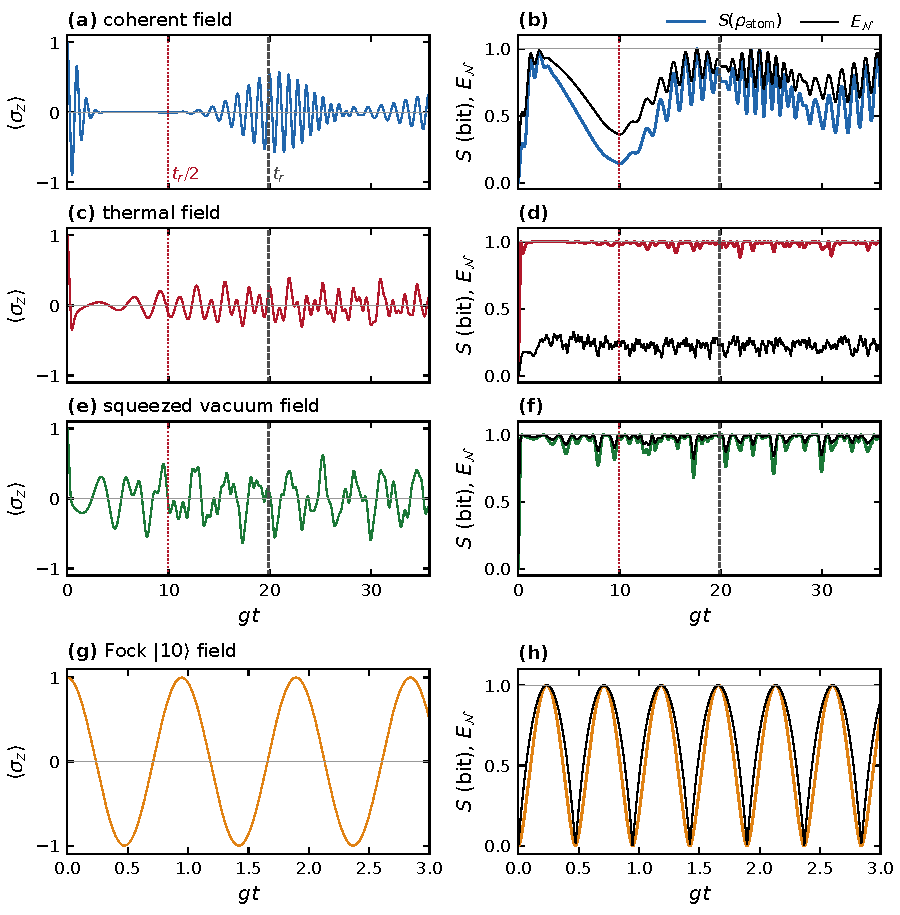
\includegraphics[width=0.92\textwidth]{fig_entanglement_comparison.pdf}
\caption{Inversion (left) and entanglement measures (right; reduced atomic entropy $S$: thick coloured line; logarithmic negativity $E_{\mathcal N}$: thin black line) for (a), (b) coherent, (c), (d) thermal, (e), (f) squeezed-vacuum and (g), (h) Fock initial fields with $\nbar = 10$. In (a)--(f) dotted and dashed vertical lines mark $t_r/2$ and $t_r$; (g) and (h) have a shorter time axis.}
\label{fig:S-states}
\end{figure}

Figure~\ref{fig:S-decoherence} shows the Wigner function at $t_r/2$ for four loss rates, and figure~\ref{fig:S-phase} the negativity and cat fidelity over the $(\nbar,\kappa/g)$ plane, from which figure~\mainref{fig:loss} was extracted.

\begin{figure}
\centering
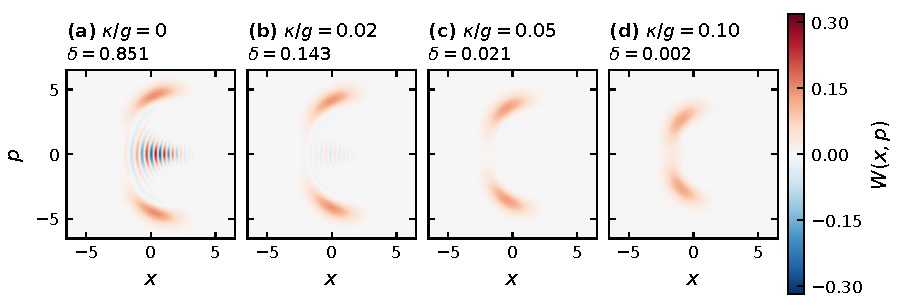
\includegraphics[width=\textwidth]{fig_wigner_decoherence.pdf}
\caption{Wigner function of the reduced field at $t_r/2$ ($\nbar = 10$) for cavity loss $\kappa/g = 0$, 0.02, 0.05 and 0.10, with the Wigner negativity $\delta$ of each state. The fringes disappear while the two components survive.}
\label{fig:S-decoherence}
\end{figure}

\begin{figure}
\centering
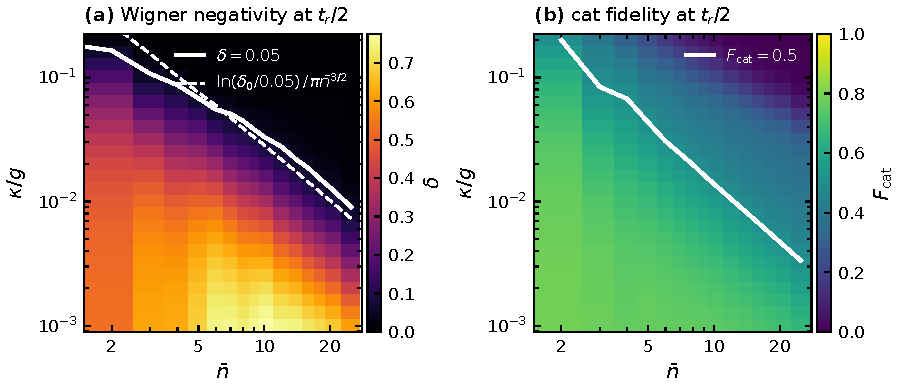
\includegraphics[width=\textwidth]{fig_phase_combined.pdf}
\caption{(a) Wigner negativity and (b) cat fidelity at $t_r/2$ over the $(\nbar,\kappa/g)$ plane. Solid white lines: $\delta = 0.05$ and $F_{\rm cat} = 0.5$. Dashed: the estimate $\ln(\delta_0/0.05)/\pi\nbar^{3/2}$.}
\label{fig:S-phase}
\end{figure}

\clearpage
\section{Notes on the exercises}

\begin{enumerate}
\item Complete the square in $(2\pi\nbar)^{-1/2}\int\exp[-u^2/2\nbar - i\mu u^2]\,du$. For $\nbar = 40$ the exact amplitudes $|Z_k|$ at $t = kt_r$ are 0.5501, 0.3958 and 0.3258 for $k = 1$, 2, 3, against $(1+\pi^2k^2)^{-1/4} = 0.5507$, 0.3965, 0.3248: agreement within 0.3\%, with the sign of the difference changing at the third revival, which overlaps its neighbours. The maxima of the envelope come later, at $t/t_r = 1.012$, 2.024 and 3.046 [compare $k\sqrt{(\nbar+1)/\nbar} = 1.012$, 2.025, 3.037], and are higher by 1.0\%, 1.2\% and 1.4\%: 0.5558, 0.4003 and 0.3304.
\item Shift the index in the second term of $P(n,t)$: $\sum_n(-1)^np_{n-1}\sin^2\theta_{n-1} = -\sum_n(-1)^np_n\sin^2\theta_n$. Equation~(\mainref{eq:parity}) gives $+0.642$, $-0.642$ and $-0.353$ for $\nbar = 9$, 10, 10.5; the exact values are $+0.641$, $-0.641$, $-0.356$.
\item See table~\ref{tab:S-squeezing} and section~S4: a variance is sensitive to the bending of the component along the circle, an overlap is not.
\item The constant is $(4+\pi^2)/32 = 0.4334$; the exact $\nbar(1-\mathcal{P})$ is 0.4023, 0.4335, 0.4335 at $\nbar = 10$, 25, 100.
\item See section~S2.3.
\item See sections~S3.3 and S3.4 and figure~\ref{fig:S-numerics}(c), (d). About ten points per fringe are needed; with an integer number the samples keep a fixed phase relative to the fringes, so the error does not average out across the envelope.
\item For the atom initially in $(\ket{e}+\ket{g})/\sqrt2 = \ket{\chi_-(0)}$ only the component $\ket{\Phi_-}$ is populated to leading order~\cite{S-gea1991}, so the state stays close to a product: no cat state and no parity revival. The rotation, the shear and the squeezing of the single component are unchanged, and the squeezing is now a property of the reduced field itself.
\end{enumerate}

\begin{thebibliography}{9}
\bibitem{S-gea1991} Gea-Banacloche J 1991 {\it Phys. Rev.} A {\bf 44} 5913
\bibitem{S-fleischhauer1993} Fleischhauer M and Schleich W P 1993 {\it Phys. Rev.} A {\bf 47} 4258
\bibitem{S-kennedy2010} Kennedy R, Horstmeyer L, Dragan A and Rudolph T 2010 {\it Phys. Rev.} A {\bf 82} 054302
\bibitem{S-gea1992} Gea-Banacloche J 1992 {\it Phys. Rev.} A {\bf 46} 7307
\bibitem{S-meunier2006} Meunier T, Le Diffon A, Ruef C, Degiovanni P and Raimond J-M 2006 {\it Phys. Rev.} A {\bf 74} 033802
\bibitem{S-gea1993} Gea-Banacloche J 1993 {\it Phys. Rev.} A {\bf 47} 2221
\bibitem{S-johansson2012} Johansson J R, Nation P D and Nori F 2012 {\it Comput. Phys. Commun.} {\bf 183} 1760
\bibitem{S-johansson2013} Johansson J R, Nation P D and Nori F 2013 {\it Comput. Phys. Commun.} {\bf 184} 1234
\bibitem{S-lambert2026} Lambert N {\it et al} 2026 {\it Phys. Rep.} {\bf 1153} 1
\end{thebibliography}

\end{document}
